\subsection{Sezioni}\label{sezioni}
Il sito risulta ampio e particolarmente denso di informazioni. Le sezioni in cui
le informazioni sono distribuite sono visualizzabili nel diagramma seguente:
    \begin{figure}[ht]
    \centering
    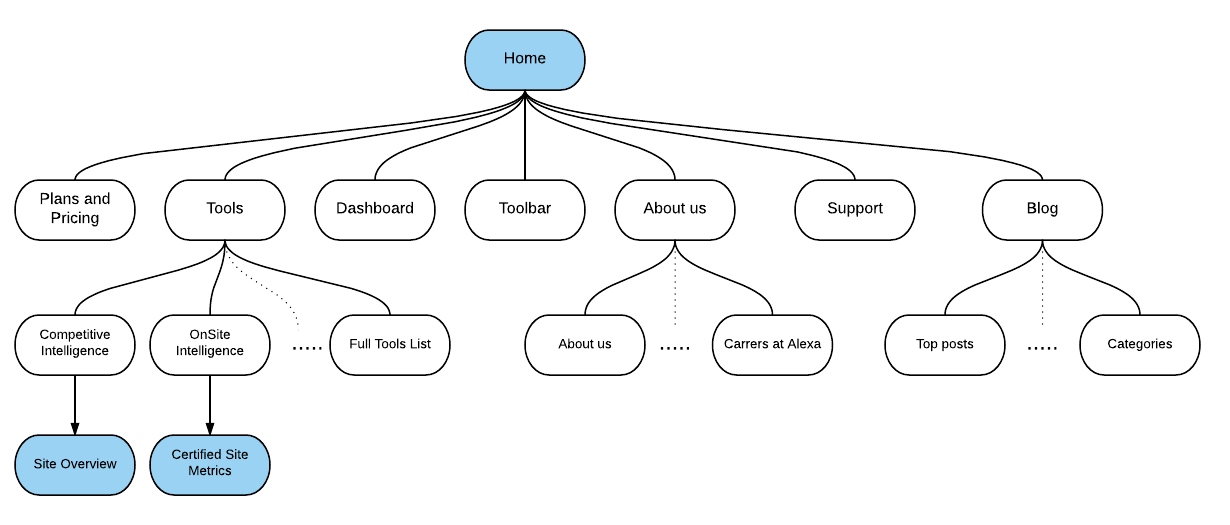
\includegraphics[scale=0.65,keepaspectratio]{{analisi/img/alexa_tree}.png}
    \caption{Struttura di alexa.com\protect\footnotemark}
    \end{figure}
    \FloatBarrier
Dal menù di navigazione il sito sembra avere un solo livello di profondità ma, analizzando attentamente ogni sezione, si nota come alcune di esse (i.e. About us) presentino una colonna a sinistra con delle voci indicanti altre sezioni. In
generale il sito risulta avere una profondità massima di livello 3.\\
Screenshot disponibile al path : \textit{Figure/2/sez0.png} \\ 
Altre sezioni sono implicitamente composte da sottosezioni presentate disponendo 
tutte le informazioni verticalmente nella 
pagina (come spiegato in §\ref{scrolling}) e permettendo l'accesso ad
altre sottosezioni attraverso dei pulsanti disseminati nella pagina stessa. 
La scelta dei pulsanti risulta poco intuitiva per l'utente anche se 
usabile: i pulsanti sono di una grandezza proporzionale alla loro 
importanza (legge di Fitts) e risultano avere un buon 
contrasto rispetto allo sfondo, oltre ad essere evidenziati nel momento in cui
vengono selezionati.
    \begin{figure}[ht]
    \centering
    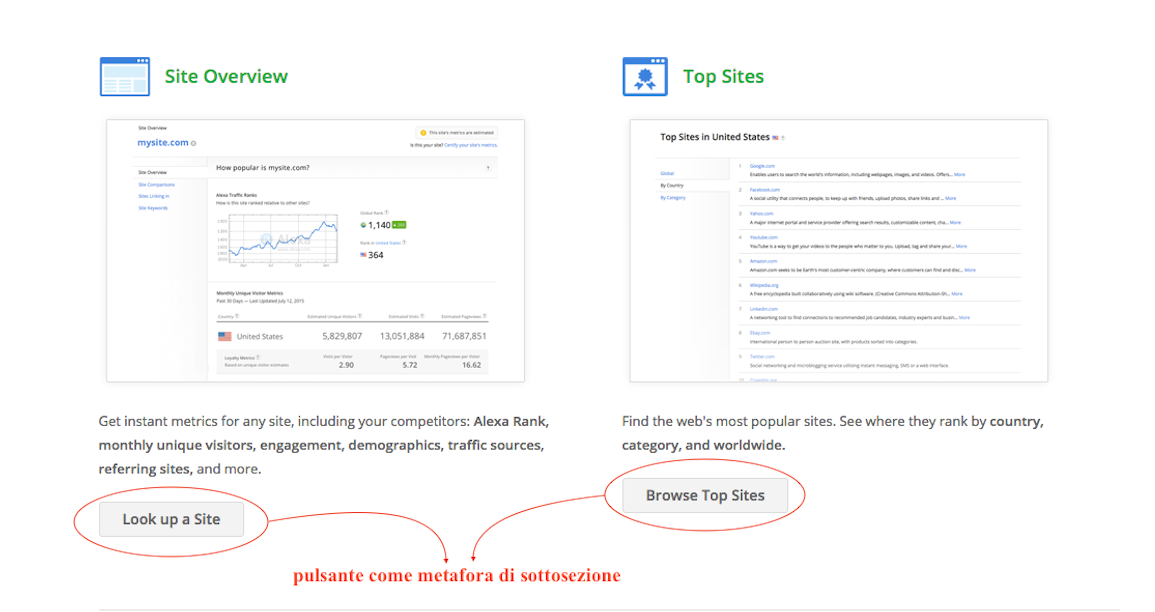
\includegraphics[scale=0.40,keepaspectratio]{{figure/2/sez1_particolare}.png}
    \caption{Pulsante come metafora di sezione di terzo livello}
    \end{figure}
    \FloatBarrier
Una nota negativa è data dalla sezione \textit{Support} 
che stravolge il layout standard eliminando totalmente il menù di navigazione e
presentando un'interfaccia che sembra essere totalmente estranea al sito, l'unico
modo per ritornare alla navigazione è cliccare sull'icona dell'azienda in alto
a sinistra che riporta alla homepage. \\
Screenshot disponibile al path : \textit{figure/2/sez2.png} \\ 
In conclusione la struttura non risulta molto chiara, anche se suddisiva in sezioni
pertinenti non aiuta l'utente ad orientarsi agevolmente all'interno del sito. \\
Risultato : \textit{5}
\footnotetext{evidenziate le sezioni analizzate in questo documento}
